\section{Мультиагентные алгоритмы} \label{ch2:ma-algs} %название по-русски

Методы обучения с подкреплением, которые специализируются на решении задач с одним агентом, плохо адаптированы для многих реальных задач, таких как автономные транспортные средства, управление водоразделом, согласованный поиск объектов, управление городским траффиком, тороговля на фондовом рынке. Поэтому необходимо расширить эти алгоритмы или даже создать новые для более сложных сценариев с настройками для нескольких агентов.

Некоторые алгоритмы, которые вдохновили эту работу, иллюстрируются в следующих разделах. Этими алгоритмами являются Multi Agent Deep Deterministic Policy Gradient \cite{lowe2017multiagent}, Counterfactual baseline for multi-agent policy gradient \cite{foerster2017counterfactual} и emergent grounded compositional language \cite{mordatch2017emergence}.

\subsection{Детерминированная политика для нескольких агентов}

Multi Agent Deep Deterministic Policy Gradient (\hyperref[acr:maddpg]{MADDPG}) -- это расширение \hyperref[acr:ddpg]{DDPG}, применяемое к настройкам нескольких агентов. Чтобы учесть все состояния среды и политики всех агентов RL в игровом сценарии, алгоритм учитывает совместные наблюдения и действия всех агентов при обучении сетей актеров и критиков. Когда дело доходит до принятия решения, сеть актора каждого агента учитывает только локальные наблюдения. Эта структура централизованного обучения и децентрализованного исполнения позволяет каждому агенту изучать оптимальную политику по консистентному градиентному сигналу. \cite{lowe2017multiagent}

\begin{figure}[ht!]
    \center
    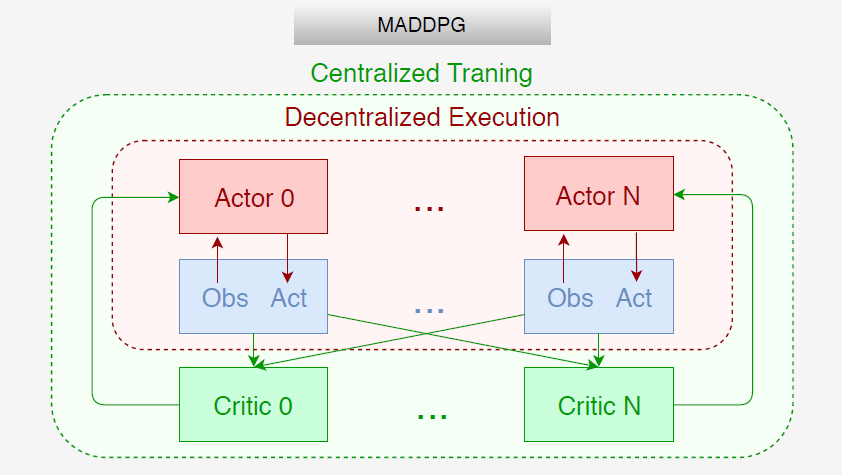
\includegraphics [scale=0.80] {my_folder/images/ch2/maddpg.png}
    \caption{у каждого агента есть децентрализованная сеть акторов, которая получает доступ только к своим локальным наблюдениям. Между тем, каждый агент имеет централизованную сеть критиков, которые имеют доступ к наблюдениям и действиям всех агентов. Критик сети обучен обновлять себя и актора. Основано на \cite{lowe2017multiagent}}
    \label{fig:ch2-maddpg}
\end{figure}

Совместные наблюдения всех агентов обозначаются через $\mathbf{x} = (o_1, ..., o_N)$, совместные действия -- через $a = (a_1, ..., a_N)$. Они вместе с наградами $r$ хранятся в буфере $D$ в виде $(\mathbf{x}, a, r, \mathbf{x}')$. Случайная выборка из $S$ выборок $(\mathbf{x}^j, a^j, r^j, \mathbf{x}'^j)$ извлекается из $D$, а критик каждого агента обновляется путем минимизации потерь:

\begin{equation}
    \begin{multlined}
        L(\theta_i) = \dfrac{1}{S} \sum_j (y^j - Q_{i}^\mu (\mathbf x^j, a_{1}^j, ...,a_{N}^j))^2
    \end{multlined}
\end{equation}

И актор обновляется семплированым градиентом политики:

\begin{equation}
    \begin{multlined}
        \nabla_{\theta_i} J \approx \dfrac{1}{S} \sum_j \nabla_{\theta_i} \mu_i (o^j_i) \nabla_{a_i} Q^\mu_i (x^j, a^j_1, ..., a_i, ..., a^j_N)|_{a_i=\mu_i(o^j_i)}
    \end{multlined}
\end{equation}

Подобно DDPG, целевые сети обновляются «мягко» на каждом шаге на $\theta' \leftarrow \tau \theta + (1 - \tau) \theta'$ с $\tau \ll 1$.

Алгоритм MADDPG хорошо подходит для сценариев с физической навигацией. Мы хотели бы продолжить изучение этого алгоритма с помощью многомерного пространства действий, особенно для сценариев, в которых агенты могут взаимодействовать при выполнении физических действий.

\subsection{Контрафактный мультиагентный градиент политики (Counterfactual Multi-Agent Policy Gradient, COMA)}

Контрафактный мультиагентный градиент политики (\hyperref[acr:coma]{COMA}) - это мультиагентный вариант метода \textit{актор-критик}, который использует единого централизованного \textit{критика} для приближения к Q-функции и отдельных децентрализованных \textit{акторов} для оптимизации политики каждого агента. \cite{foerster2017counterfactual}

В кооперативных задачах с несколькими агентами сложность сотрудничества возрастает с увеличением количества агентов. Таким образом, было бы нецелесообразно и неэффективно иметь одну единственную оптимальную политику для всех агентов. Вместо этого децентрализованные политики для каждого агента формулируются в виде проблем с несколькими агентами. В COMA один централизованный критик и отдельные акторы тренируются совместными действиями и совместными наблюдениями. Когда дело доходит до исполнения, каждый актор генерирует действия на основе собственной истории наблюдения, см. \firef{fig:ch2-coma}.

\begin{figure}[ht!]
    \center
    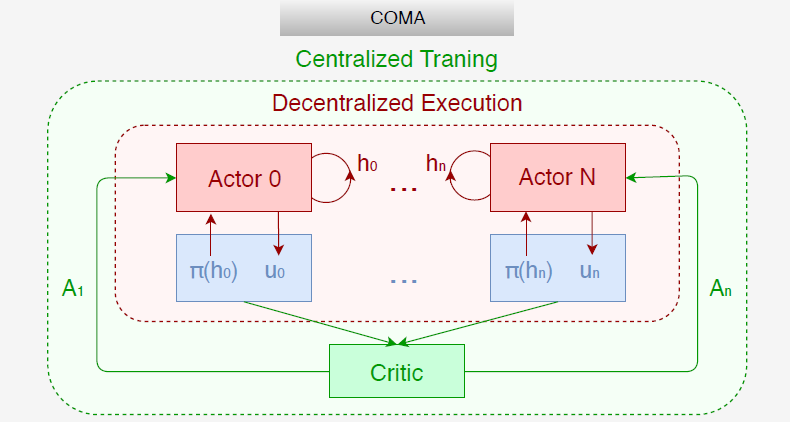
\includegraphics [scale=0.80] {my_folder/images/ch2/coma.png}
    \caption{Структура сетей алгоритма COMA и информационный поток между централизованным критиком и децентрализованными акторами. В COMA отдельно происходит обучение одного централизованного критика и каждого из акторов. Каждый актор децентрализован, при принятии решений использует локальные истории наблюдения. \cite{foerster2017counterfactual}}
    \label{fig:ch2-coma}
\end{figure}

COMA предназначен для мультиагентных совместных сценариев с глобальной функцией награды для всех агентов. Однако агенты, обученные COMA, изучают отдельные политики без явного общения. \cite{foerster2017counterfactual}

\subsection{Возникающий язык (Emergent Language)}

Grounded compositional language обозначает простой язык, где агенты связывают конкретные символы с конкретными объектами, а затем объединяют эти символы в значимые понятия \cite{Szabo2008-SZAC}. Язык представлен в виде абстрактных дискретных символов, произнесенных агентами, которые не имеют заранее определённого значения, но возникли и сформировались в процессе обучения в соответствии со средой и целями \cite{mordatch2017emergence}. В отличие от естественного языка, для работы с которым извлекаются языковые шаблоны из большого набора текстовых данных, этот язык, возникший во время обучения с подкреплением, понятен только агентам и используется ими для сотрудничества друг с другом в достижении общих целей.
